\textbf{Modify the code \textsc{fluidflow.m} to solve the equations 
\begin{align*}
\omega_t+\psi_y\omega_x-\psi_x\omega_y &= Pr\Delta\omega+RaPrT_x,\\
T_t+\psi_yT_x-\psi_xT_y &= \Delta T,\\
\Delta\psi &= -\omega,
\end{align*}
where $(x,y)\in (0,1)\times (0,1)$ and $t>0$. Here $\omega$ is the fluid vorticity, $\psi$ the stream function and $T$ the temperature. The independent non-dimensional constants are the Rayleigh number $Ra$, which reflects the buoyant contribution, and the Prandtl number $Pr$, which is the ratio of viscous to thermal diffusion. For this exercise, set to $Ra = 2\cdot 10^5$ and $Pr=0.71$ (air). The fluid is at rest at $t= 0$, with $T=\psi=\omega= 0$. The boundary condition for the stream function is $\left.\psi\right|_{\Gamma}=0$, which implies that there is no mass transfer through the boundary $\Gamma$. The value of the vorticity at the walls is expressed as $\omega_{\Gamma}=-\left.\Delta\psi\right|_{\Gamma}$ and the temperature at $\Gamma$ is defined by
\begin{align*}
T(t,x,y) = 
\begin{cases}
       2^9\tanh^4(100t)x^5(x-1)^4,&  y=0, x\in [0,1], t>0,\\
       0,& (x,y)\in\Gamma, y\neq 0, t>0.
\end{cases}
\end{align*}
}
\newline

We first compute the vorticity from the velocity field,
\begin{align*}
\omega = vD_p-Du,
\end{align*}
where $D_p$ is the transpose of $D$, the Chebyshev differentiation matrix. Then we advance the vorticity and the temperature,
\begin{align*}
\omega &= \omega + \Delta t\left[-v.D\omega-u.\omega D_p+Pr\left(wD_{2p}+D_2\omega\right)+RaPrTD_p\right],\\
T &= T + \Delta t\left[-v.DT-u.TD_p+TD_{2p}+D_2T\right].
\end{align*}
Further, we recompute the stream function in the interior (the exterior keeps being zero). To solve the Poisson equation we are going to use the Sylvester equation and algorithm instead of LU factorization (see figures 6 and 7 for comparison between the two methods).
\begin{align*}
D_2\psi+\psi D_{2p}&=-w,\\
A\psi+\psi B &= C.
\end{align*}
To finish, we recalculate the velocities from the streamfunction,
\begin{align*}
u &= D\psi,\\
v &= -\psi D_{p},
\end{align*}
and impose boundary conditions on the velocities and the temperature,
\begin{align*}
u_{\Gamma}&=0,\\
v_{\Gamma}&=0,\\
T_{\Gamma}&=0,\\
T_{\Gamma}(t,x,y= 0)&=2^9\tanh^4(100t)x^5(x-1)^4.
\end{align*}

In the following figure we show the ratio between the time spent in solving the Poisson equation using LU factorization and Sylvester's algorithm versus the number of iterations. The red lines indicate the average and the standard deviation of the date. We can see that using Sylvester's equation leads to an improvement of a factor greater than 3. In figure 7 we can see the difference in the solutions is of the order of $10^{-11}$, concluding that it is advisable for this problem to use the Sylvester's approach to solve the Poisson equation. 

\begin{figure}[H]
\centering
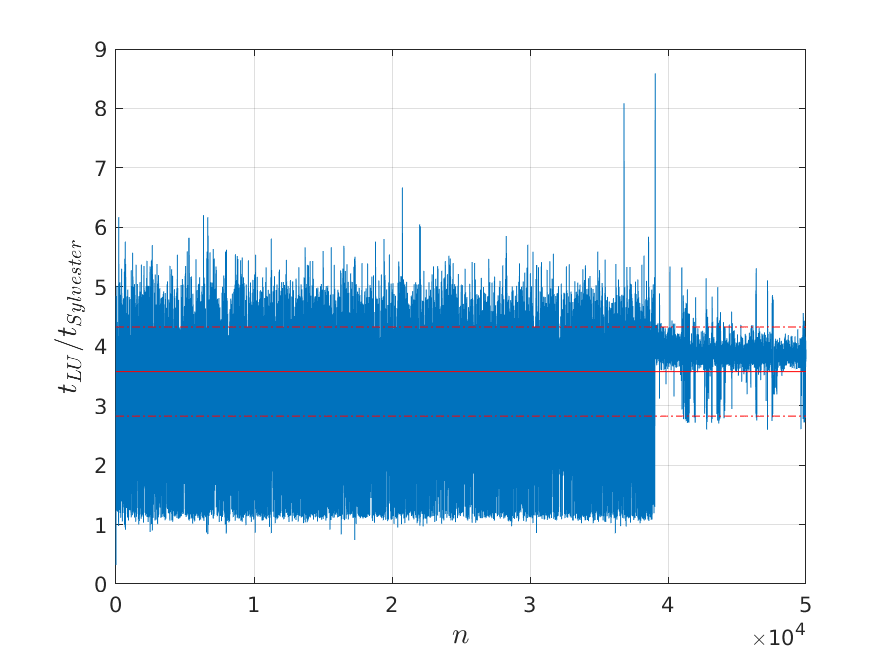
\includegraphics[scale=0.9]{P5_comparison.png}\caption{Performance comparison between LU and Sylvester's algorithm for the Poisson equation.}
\end{figure}

\begin{figure}[H]
\centering
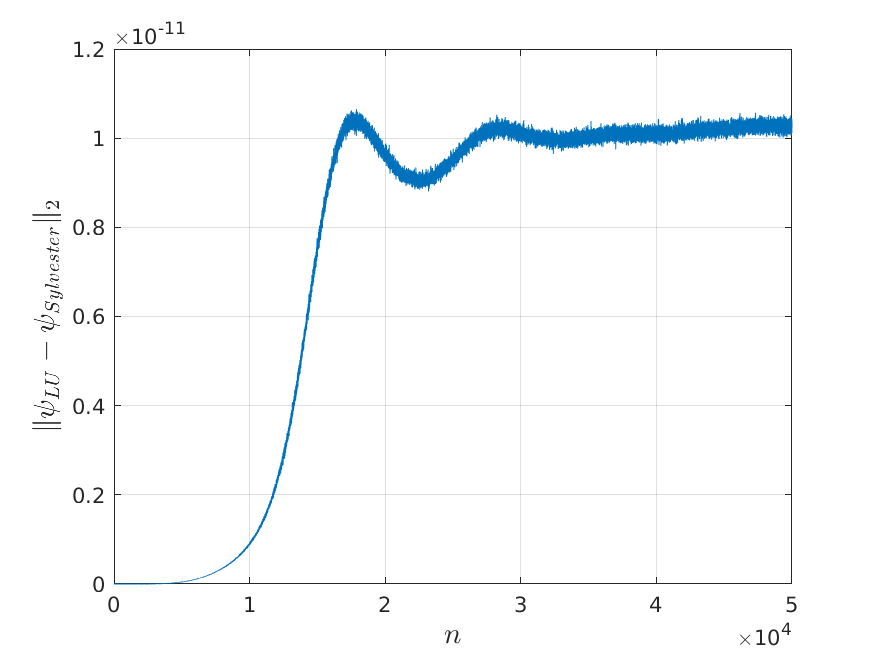
\includegraphics[scale=0.9]{P5_diff.png}\caption{Differnce between the $\psi$ obtained using LU and Sylvester's algorithm.}
\end{figure}

In the next figure we see how the natural convection makes the fluid move. The hot floor makes the fluid ascend and given the no divergence condition and the non-uniformity of the temperature at the base, it is forced to rotate as we can see from the streamlines, vorcitity and velocity fields. We can see a very different situation if the hot surface is placed on top. Given the blocked convection the fluid would not move as much, as we see in figure 9. We can still see that the fluid moves, but its movement is confined to the upper part of the domain. This results are at $t=0.1$.

\begin{figure}[H]
\centering
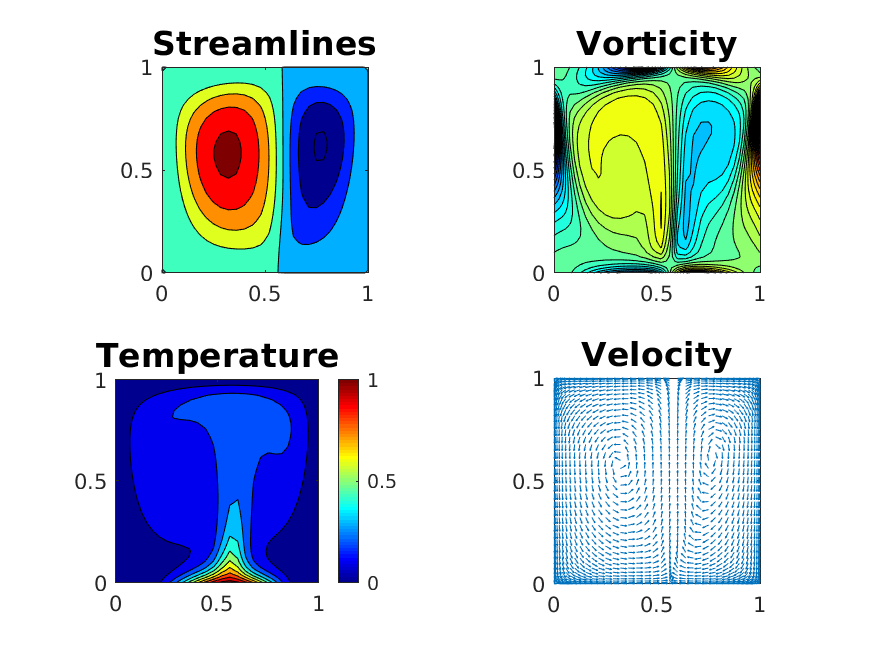
\includegraphics[scale=1.2]{P5.png}\caption{Results obtained for natural convection at $t=0.1$.}
\end{figure}

\begin{figure}[H]
\centering
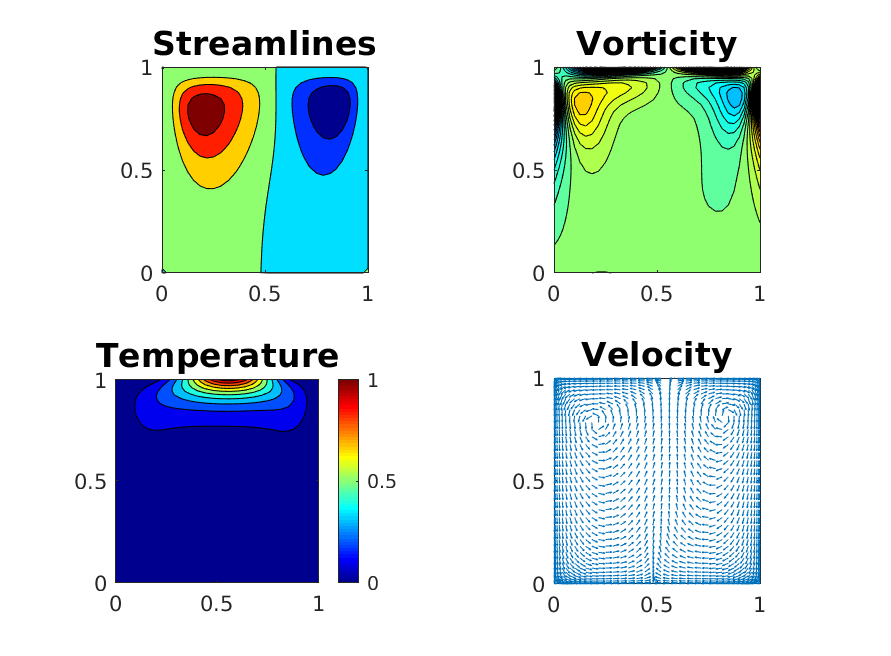
\includegraphics[scale=1.2]{P5_blocked.png}\caption{Results obtained for blocked convection at $t=0.1$.}
\end{figure}

\subsection*{Matlab code for this problem}

\begin{verbatim}
%% Homework 4, Problem 5 -  Francisco Castillo
clear all; close all; clc;

% Parameters
N = 40;  %40
Pr = 0.71;
Ra = 2e5;
dt = 2e-6;
 
% Grid and diff matrices
[D,xch] = cheb(N-1);
x = (-xch+1)/2; D = -2*D;   % To trasnlate the domain to [0,1]
[xx,yy] = meshgrid(x);

Dp = D';
D2 = D^2; D2p = D2';
indb = find(xx==0|xx==1|yy==0|yy==1); % For what?? Impose BCs in velocities
 

% Laplacian of the interior
L = kron(eye(N-2),D2(2:end-1,2:end-1))+kron(D2(2:end-1,2:end-1),eye(N-2));  
%Linv = inv(L);
[lo,up,per] = lu(L,'vector');  % LU factorization
 
% Initial velocity & pre-allocate memory
T = 0*xx;
psi = T;
psi2 = T;
w = T;
u = T;
v = T;
% Everything initialized to zero
count = 0;
t = 0;

% boundary condition
Topt = 'blocked convection';
if (strcmp(Topt,'natural convection'))
    T(1,:) = TempBC(t,x);
elseif (strcmp(Topt,'blocked convection'))
	T(end,:) = TempBC(t,x);
end

% main loop
i=0;
while t<.1%200
    i=i+1;
    % vorticity 
    w = v*Dp-D*u;  % w = dvdx-dudy

    % Advance Vorticity
    w =  w + dt*(-v.*(D*w)-u.*(w*Dp)+Pr*(w*D2p+D2*w)+Ra*Pr*T*Dp);

    % Advance Temperature
    T = T + dt*(-v.*(D*T)-u.*(T*Dp)+T*D2p+D2*T);

    % compute stream function
    %    tic 
    %    wi = w(2:end-1,2:end-1); wi=wi(:);
    %    psi(2:end-1,2:end-1) = reshape(up\(lo\(-wi(per))),N-2,N-2);
    %    time1(i) = toc;
    %    tic
    psi(2:end-1,2:end-1) = sylvester(D2(2:end-1,2:end-1),D2p(2:end-1,2:end-1),-w(2:end-1,2:end-1));
    %    time2(i) = toc;
    %    diff(i) = norm(psi-psi2);

    % Update Velocity
    u = D*psi;
    v = -psi*Dp;

    % BC's for u,v,T. Vorticity is calculated from u,v. Stream-function is
    % obtained from w.
    u(indb) = 0;
    v(indb) = 0;
    T(:,1) = 0;
    T(:,end) = 0;
    if (strcmp(Topt,'natural convection'))
        T(1,:) = TempBC(t,x); 
        T(end,:) = 0;
    elseif (strcmp(Topt,'blocked convection'))
        T(1,:) = 0;
        T(end,:) = TempBC(t,x);
    end

    % Advance time
    t = t+dt;

   count = count + 1;
   if count == 200
       
       subplot(2,2,1)
       contourf(xx,yy,psi)
       axis([0 1 0 1]), axis square
       colormap(hot)
       title('Streamlines','fontsize',16)
        
       subplot(2,2,2)
       contourf(xx,yy,w,30)
       axis([0 1 0 1]), axis square
       title('Vorticity','fontsize',16)
      
       subplot(2,2,3)
       contourf(xx,yy,T)
       axis([0 1 0 1]), axis square
       title('Temperature','fontsize',16)
       colormap(jet)
       colorbar
       caxis([0 1])
       
       speed = sqrt(u.^2+v.^2);
       
       subplot(2,2,4)
       quiver(xx,yy,u./speed,v./speed)
       axis([0 1 0 1]), axis square
       title('Velocity','fontsize',16)
       
       drawnow
              
       count = 0;
   end

end
if (strcmp(Topt,'natural convection'))
    saveas(gcf,'Latex/FIGURES/P5','png')
elseif (strcmp(Topt,'blocked convection'))
    saveas(gcf,'Latex/FIGURES/P5_blocked','png')
end

%%
% n = 1:i;
% figure
% plot(n,time1./time2)
% hold on
% plot(n,mean(time1./time2)*ones(size(n)),'r')
% plot(n,(mean(time1./time2)+std(time1./time2))*ones(size(n)),'r-.')
% plot(n,(mean(time1./time2)-std(time1./time2))*ones(size(n)),'r-.')
% grid on
% xlim([0 n(end)])
% xlabel('$n$','interpreter','latex','fontsize',14)
% ylabel('$time_1/time_2$','interpreter','latex','fontsize',14)
% ylabel('$t_{LU}/t_{Sylvester}$','interpreter','latex','fontsize',14)
% saveas(gcf,'Latex/FIGURES/P5_comparison','png')
% 
% figure
% plot(n,diff)
% grid on
% xlabel('$n$','interpreter','latex','fontsize',14)
% ylabel('$\|\psi_{LU}-\psi_{Sylvester}\|$','interpreter','latex','fontsize',14)
% ylabel('$\|\psi_{LU}-\psi_{Sylvester}\|_2$','interpreter','latex','fontsize',14)
% xlim([0 n(end)])
% saveas(gcf,'Latex/FIGURES/P5_diff','png')


function Ty0 = TempBC(t,x)
    Ty0 = 2^9*(tanh(100*t))^4*x.^5.*(x-1).^4;
end
\end{verbatim}